\documentclass[arhiv]{../izpit}
\usepackage{fouriernc}
\usepackage{xcolor}
\usepackage{tikz}
\usepackage{fancyvrb}
\usetikzlibrary{calc,shapes.multipart,chains,arrows}
\VerbatimFootnotes{}

\begin{document}
	
	\izpit{Programiranje I: 1. Izpit}{28.\ januar 2020}{
		Čas reševanja je 150 minut.
		Veliko uspeha!
	}
	
	%%%%%%%%%%%%%%%%%%%%%%%%%%%%%%%%%%%%%%%%%%%%%%%%%%%%%%%%%%%%%%%%%%%%%%%
	
	V nalogah si lahko pomagate z rešitvami prejšnjih nalog.
	
	\naloga 
	
	\podnaloga Definirajte funkcijo \verb|option_sum: int option -> int option -> int option|, ki vrne vsoto argumentov, če je to mogoče, ali pa \verb|None|, če je katerikoli od argumentov \verb|None|.
	\begin{verbatim}
	# option_sum (Some 1) None;;
	- : int option : None
	\end{verbatim}
	
	\podnaloga Imamo funkcijo \verb|strange_map f l r x|, kjer velja: \verb|f: ('a -> 'b * 'c)|, \verb|l: ('b -> 'd)|, \verb|r: ('c -> 'e)| in \verb|x : 'a|. Funkcija \verb|x| s funkcijo \verb|f| preslika v par in na komponentah ustrezno uporabi \verb|l| in \verb|r|. Definirajte ustrezno funkcijo.
	
	\podnaloga Definirajte funkcijo \verb|function_repeat: ('a -> int) -> 'a list -> 'a list|, ki sprejme funkcijo \verb|f| in seznam ter vrne nov seznam, kjer se posamezen element \verb|x| iz začetnega seznama ponovi \verb|f x| krat. Nepozitivne ponvitve pomenijo, da elementa v končnem seznamu ni. Za vse točke naj bo funkcija repno rekurzivna, kar tudi argumentirajte.
	\begin{verbatim}
	# function_repeat (fun x -> x) [0;1;2;(-2)];;
	- : int list = [1;2;2]
	\end{verbatim}
	
	
	\podnaloga Definirajte funkcijo \verb|iterate: ('a -> 'a) -> ('a -> bool) -> 'a -> 'a|, ki sprejme funkcijo za iteriranje, zaustavitveni pogoj in začetno vrednost. Funkcija naj funkcijo za iteriranje zaporedoma uporablja, dokler ne velja zaustavitveni pogoj. Funkcija naj vrne prvi rezultat, pri katerem zaustavitveni pogoj vrne \verb|true|.
	
	\begin{verbatim}
	# iterate (fun x -> 0.5*.(x+.10.0/.x)) (fun x -> abs_float(x*.x-.10.0)<0.01) 10.0;;
	- : float = 3.16245562280389
	\end{verbatim}
	
	\naloga
	\textit{Napreden povezan seznam} je podoben običajnemu seznamu v OCaml-u, le da imamo namesto ene vrednosti v posameznem vozlišču tabelo, ki lahko vsebuje več elementov (velikosti niso nujno enake). Enako kot običajen povezan seznam je sestavljen in dveh različnih gradnikov: praznega seznama in vozlišča s tabelo in preostankom seznama.
	
	
	\podnaloga Definirajte polimorfen tip \verb|'a improved_list| ter seznam \verb|test : int improved_list|, ki predstavlja spodnji izboljšan seznam:
	% Stolen from https://tex.stackexchange.com/questions/19286/how-should-i-draw-a-singly-double-linked-list
	\[
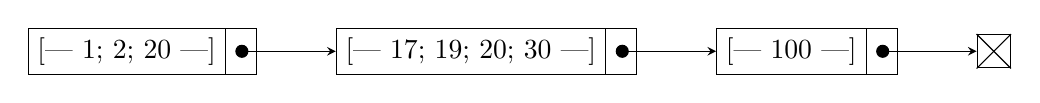
\begin{tikzpicture}[list/.style={rectangle split, rectangle split parts=2,
	draw, rectangle split horizontal}, >=stealth, start chain]

\node[list,on chain] (A) {[| 1; 2; 20 |]};
\node[list,on chain] (B) {[| 17; 19; 20; 30 |]};
\node[list,on chain] (C) {[| 100 |]};
\node[on chain,draw,inner sep=6pt] (D) {};
\draw (D.north east) -- (D.south west);
\draw (D.north west) -- (D.south east);
\draw[*->] let \p1 = (A.two), \p2 = (A.center) in (\x1,\y2) -- (B);
\draw[*->] let \p1 = (B.two), \p2 = (B.center) in (\x1,\y2) -- (C);
\draw[*->] let \p1 = (C.two), \p2 = (C.center) in (\x1,\y2) -- (D);
\end{tikzpicture}
	\]
	
	\podnaloga Definirajte funkcijo \verb|len: 'a improved_list -> int|, ki vrne dolžino podanega seznama.
	
		
	\podnaloga Definirajte funkcijo \verb|index: 'a improved_list -> int -> 'a option|, ki vrne i-ti element, ali \verb|None|, če le ta ne obstaja. Za vse točke mora biti funkcija repno rekurzivna.
	
	\begin{verbatim}
	# index test 5;;
	- : int option = Some 20
	\end{verbatim}
	
	\podnaloga Definirajte funkcijo \verb|is_sorted: ('a -> 'a -> bool) -> 'a improved_list -> bool|, ki sprejme funkcijo primerjanja in vrne \verb|true|, če je napreden seznam urejen glede na to funkcijo. Za vse točke mora biti funkcija repno rekurzivna in imeti linearno časovno zahtevnost.
	
	\begin{verbatim}
	# is_sorted (<=) test;;
	- : bool = false
	\end{verbatim}
	
	\podnaloga Definirajte funkcijo \verb|update: 'a improved_list -> int -> 'a -> 'a improved_list|, ki vrne nov izboljšan seznam, kjer vrednost na indeksu drugega argumenta nadomesti z vrednostjo tretjega argumenta. Če je indeks nesmiselen, naj funkcije vrne kar originalni seznam. Pazite, da pri tem originalni seznam ostane nespremenjen. Za vse točke mora biti funkcija repno rekurzivna, kar v komentarju tudi argumentirajte.
	
	\begin{verbatim}
	# index (update test 5 (-3)) 5;;
	- : int option = Some (-3)
	# index test 5;;
	- : int option = Some 20
	\end{verbatim}
	
	\naloga
	% blocky(n,m,l)
	\podnaloga Na mizo dolžine $n$ si želimo postaviti dekoracijo iz $m$ pravokotnih posod za rože, kjer je vsaka posoda dolžine $l$. Posode za rože postavljamo eno za drugo, med dvema zaporednima posodama pa mora biti vsaj 1 enota mize prazna. Sestavite funkcijo, ki sprejme $n$, $m$ in $l$ in vrne število različnih postavitev posod za rože na mizo, kjer moramo vedno porabiti vse posode in posod med seboj ne razlikujemo.
	
	\podnaloga Dolžine korit so lahko različne. Sestavite funkcijo, ki sprejme število $m$ in seznam celih števil, ki predstavlja dolžine posod za rože in vrne število različnih postavitev posod na mizo, kjer je vrstni red korit določen z vrstnim redom v podanem seznamu. (Ta podnaloga je lažja oblika prejšnje, če je rešitev popolnoma pravilno šteje tudi kot pravilna rešitev prejšnje podnaloge.)
	
	
\end{document}